\vspace{-0.5cm}
\section{Introduction}
The human brain has been a subject of extensive research by the medical image community with a wide range of objectives, from practical clinical applications like disease diagnosis and surgical planning, to addressing scientific questions related to its structure and function. The goal of brain image registration is to compute a transformation that brings images of the brain into anatomical correspondence. We can classify volumetric image registration methods according to two main criteria: a) the deformation model \textcolor{red}{(rigid/non-rigid)}, and b) the similarity measure (mono-modal/multi-modal). Registration of images from different modalities (\emph{multi-modal} image registration) is a specially challenging task, since an appropriate similarity metric is harder to define in the multi-modal case than in the \emph{mono-modal} case. Multi-modal image registration \textcolor{red}{is often constrained to rigid transforms \cite{DeNigris2012, Orchard2008, Orchard2010, Maes1997, Roche1998}}. Since registration of medical images of different modalities is almost exclusively applied to intra-subject image registration, it is often \textcolor{red}{assumed that there exists rigid} transformation that correctly brings them into correspondence. However, certain imaging modalities present severe distortions that cannot be accommodated by a \textcolor{red}{rigid transform}. Consider for example the case of Echo Planar Images (EPI), which suffer from distortions caused by magnetic field inhomogeneities \cite{Tournier2011, Andersson2003}. In Fig. \ref{fig:example_t1b0_problem} we show an example of two $B_{0}$ EPI images (from a dwMRI dataset) with opposite phase encode directions and a T1-weighted image from the same subject. The noticeable geometric distortions in the $B_{0}$ images are caused by differences in the magnetic susceptibility of different tissue types of the brain. These geometric distortions make their registration to the T1 image (even being from the same subject), a \textcolor{red}{non-rigid registration} problem if these artifacts are not corrected beforehand \cite{Bhushan2015}. Although several correction methods have been proposed to correct geometric distortions in EPI \cite{Andersson2003, Holland2010, Ruthotto, Irfanoglu2015}, most of them require at least two images acquired with opposite phase-encode directions. If such extra images are not available, for example in data sets which were acquired without considering the need for correction, then the images cannot be corrected prior to registration with the T1. Despite the complexity of this registration task, it has a wide range of potential applications. Combining diffusion data with T1 MRI, for instance, has the potential of significantly improving tractography \cite{Smith2012, Girard2014}. Besides diffusion MRI, the development of \textcolor{red}{non-rigid} multimodal registration methods has the potential to impact other image modalities, like functional MRI (which are also affected by susceptibility-induced geometric distortions), and intra-operative ultrasound images, which capture the deformation of the brain as a result of brain surgery \cite{Rivaz2015, DeNigris2012}.


\begin{figure}[t!]
%\centering
%    \subfloat[]{\label{fig:T1B0_task_example_b0_up}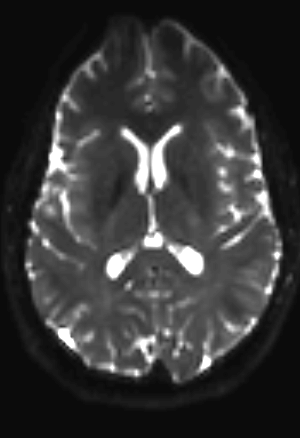
\includegraphics[width=0.3\linewidth]{images/T1B0Result/T1B0_task_example_b0_up_enhanced.png}}
%    \subfloat[]{\label{fig:T1B0_task_example_b0_down}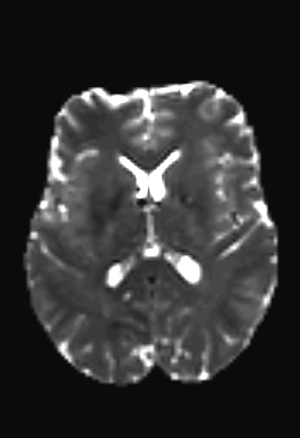
\includegraphics[width=0.3\linewidth]{images/T1B0Result/T1B0_task_example_b0_down_enhanced.png}}
%    \subfloat[]{\label{fig:T1B0_task_example_t1}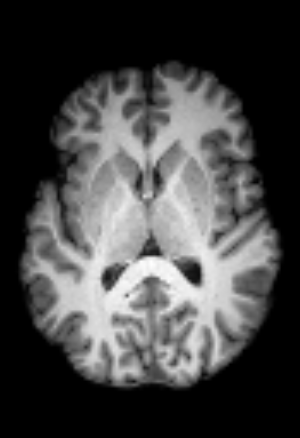
\includegraphics[width=0.3\linewidth]{images/T1B0Result/T1B0_task_example_t1.png}}
%    \closer
%    \caption{{\small Two $B_{0}$ images with opposite phase-encode blips (a,b) and a T1 (c) from the same subject, acquired in the same session.}}
%\label{fig:example_t1b0_problem}\figcloser
%\end{figure}
\centering
    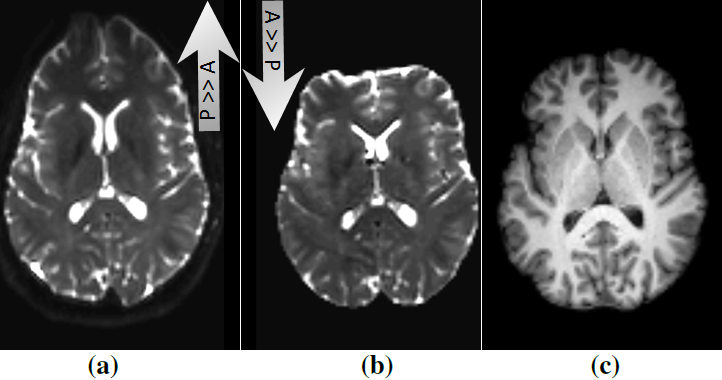
\includegraphics[width=1\linewidth]{images/T1B0Result/figure1.png}
    \closer
    \caption{{\small Example of a multi-modal, \textcolor{red}{non-rigid}, registration problem. (a,b) Two $B_{0}$ images with opposite phase-encode directions and (c) a T1-weighted image from the same subject. If both $B_{0}$ images are available, then the $B_{0}$ and T1-weighted images can be rigidly registered after the \textcolor{red}{geometric} distortions have been corrected. However, if only one of the $B_{0}$ images is available, traditional correction algorithms are not applicable and co-registration of the distorted $B_{0}$ with the T1-weighted image is a \textcolor{red}{non-rigid} registration problem.}}
\label{fig:example_t1b0_problem}\figcloser
\end{figure}
\vspace{-0.4cm}
\subsection{Information theoretic measures}
Existing multi-modal registration methods may be classified into two main approaches: 1) optimize information theoretic measures from the estimated joint probability distribution function (PDF), 2) reduce the multi-modal problem to the mono-modal case. The most prominent example of metrics based in information theory is mutual information (MI) \cite{Maes1997, Mattes2003}. The success of MI is explained by its generality, since it does not assume the existence of a functional relationship between the intensities in the two modalities. This generality comes at the expense of disregarding any notion of proximity of intensity values: two intensities will be considered similar only if their estimated joint PDF is high, no matter how close they are numerically, which may cause a large number of local maxima (see Fig. 2 in Roche {\it et al.}, 1998 \cite{Roche1998}). In the standard formulation of MI, the joint PDF is estimated from the whole image ({\it i.e.}, it is a {\it global} metric), which makes the metric more robust to the effects of noise \cite{Mattes2003}. An important limitation of this kind of global metrics is that the globally estimated PDF cannot capture non-stationary relationships between image intensities \cite{Hermosillo2004}. \textcolor{red}{Orchard \cite{Orchard2008} exploits the well known property that good intensity correspondences are directly related to compact clusters in the joint intensity scatter plot (JISP) \cite{Hermosillo2004}
to directly formulate the registration problem as clustering in the JISP using line segments and points to model two possible cluster shapes. Since the resulting metric is based on the globally computed JISP, this approach shares some of the limitations of MI previously mentioned. Orchard and Mann \cite{Orchard2010} developed a method to simultaneously register two or more images by parameterizing the (global) joint intensity distribution using a Gaussian Mixture Model (GMM), which simplifies the estimation of the GMM parameters by maximum likelihood.} A direct approach to tackle \textcolor{red}{the problem of non-stationary intensity correspondences} is to use locally estimated probability functions. Hermosillo {\it et al.} \cite{Hermosillo2004}, for instance, estimates the joint PDF locally by using Gaussian kernels centered at each voxel as weighting functions to reduce the contribution of far voxels. A limitation of this strategy, however, is its computational cost, as pointed out by Hermosillo \cite{Hermosillo2004}, since it results in a separate PDF estimation for each pixel, which makes it necessary to perform some simplifications. Besides, as we reduce the number of local samples, the estimation becomes more sensitive to noise~\cite{Mattes2003}.

\vspace{-0.2cm}
\subsection{Reduction to the mono-modal case}
Reducing the multi-modal problem to the mono-modal case may be accomplished by assuming the existence of a {\it transfer function} between the two modalities (a function that maps intensity values of one modality to corresponding intensities in the other). Although this strong assumption is not satisfied in general, experimental results have shown that it is not critical for typical brain image registration tasks~\cite{Roche1998}. Roche {\it et al.} \cite{Roche2000} showed that, assuming the existence of a transfer function, a maximum-likelihood formulation of the registration problem is equivalent to maximization of the correlation ratio (CR). Being a global metric, CR shares the robustness to noise of MI but also the inability to capture non-stationary relationships between image intensities. However, one of the advantages of CR over MI is that it is sensitive to proximity of intensity values, which may help to reduce the number of local maxima \cite{Roche1998}. An additional advantage is that CR can be computed efficiently from statistics from the images' iso-sets instead of explicitly estimating the joint PDF. \textcolor{red}{ Guimond et al. \cite{Guimond2001} assume that the intensity correspondence can be described by at most two polynomial functions. By reducing the degrees of freedom to polynomials, the resulting transfer function is reported to be robust enough to be used for elastic registration, in contrast to CR which was designed for parametric (rigid/affine) registration.} Arce {\it et al.} \cite{Arce-santana2014} proposed a similar formulation of the registration problem which also makes the functional dependency assumption. In their work, the transfer function is modeled as a set of hidden random variables whose values can be estimated using the Expectation Maximization (EM) algorithm. Since the assumptions are similar to those made by Roche {\it et al.} \cite{Roche1998, Roche2000}, the resulting optimal transfer functions are the same. However, the resulting metric differs in that it introduces a measure of uncertainty for each intensity value, which helps to alleviate the effect of non-functional and non-stationary distributions.\\

Recently, Bhushan {\it et al.} \cite{Bhushan2015} proposed an algorithm, called INVERSION, for T1-$B_{0}$ co-registration in the presence of susceptibility induced distortions. In their work, the $B_0$ to T1 transfer function is assumed to be monotonically decreasing and is computed by matching the intensity histograms of the input images. The main novelty of INVERSION is that the transfer function is applied to the $B_0$ after its intensities have been modulated with the local Jacobian of the transformation (eq. 5 in \cite{Bhushan2015}). However, since the transformation is not constrained to be diffeomorphic (as opposed to recent correction techniques \cite{Ruthotto, Irfanoglu2015}), the local Jacobian does not necessarily correspond to a transform explaining plausible geometric distortions \cite{Chang1992}. Also, since it is computed only from the histograms of the input images, the resulting transfer function may not be accurate enough, and the authors propose to refine the result using Normalized Mutual Information.

%One of the limitations of the original formulation proposed by Arce {\it et al.} \cite{Arce-santana2014} is that it is asymmetric (a limitation shared with CR) in the sense that the transfer function to be estimated must be chosen beforehand (to either map intensities from modality A to modality B or viceversa), which may result in very different solutions.
%Another limitation is that Arce {\it et al.} \cite{Arce-santana2014} use an elastic deformation model \cite{Bajcsy1982, Gee1999}, and their optimization strategy consists in a Gauss-Newton iterative algorithm \cite{GVK502988711} that requires to solve a series of large systems of linear equations.

\vspace{-0.2cm}
\subsection{Quantitative evaluation}
Validation is one of the most challenging aspects in image registration. The most accepted validation methodologies, in the mono-modal case, consist in measuring the overlap of manually annotated anatomical regions \cite{Klein2009, Klein2010, Rohlfing2012}. These methodologies have made possible to quantitatively evaluate \textcolor{red}{non-rigid} registration algorithms and compare their performance in a meaningful way. However, to the best of our knowledge, there are no equivalent studies that quantitatively evaluate the accuracy of \textcolor{red}{non-rigid} registration algorithms in the multi-modal case. In practice, performance is assessed only visually. The reason why validation becomes more challenging in the multi-modal case is that, as far as we know, there are no manually annotated multi-modal image sets publicly available.
%The Symmetric Normalization (SyN) algorithm developed by Avants {\it et al.} \cite{Avants2008, Avants2011}, and made available as part of the Advanced Normalization Tools (ANTS) %\cite{Avants2011a}, has been extensively tested in large comparative studies using the aforementioned methodologies and has consistently been reported as one of the most %accurate. For multi-modal images, the MI metric is implemented in ANTS, and can be used with SyN for diffeomorphic registration.

\vspace{-0.2cm}
\subsection{Summary of contributions}
Our contributions are two-fold:
\begin{enumerate}
\item{We propose a new matching functional for \textcolor{red}{non-rigid} multi-modal brain MRI registration. Our model is based on the empirical observation (explained in detail in section \ref{sec:methods}) that the \textbf{non-linear, local} \textcolor{red}{intensity correspondence} between both modalities may be made closer to linear by applying a \textbf{global, non-linear} transfer function. We prove that the maximum likelihood estimator of the transfer function coincides (under mild assumptions) with the optimal transfer function used in the CR and EM functionals \cite{Roche1998, Arce-santana2014, Ocegueda2015}. The resulting functional, which we call Expected Cross Correlation (ECC) may be regarded as an extension to Cross Correlation (CC) to the multi-modal case. By estimating both transfer functions between image modalities, we eliminate the need for an image modality to be chosen {\it a priori}. Our symmetric formulation allows us to naturally implement our matching functional into the SyN \cite{Avants2011a} algorithm.}
\item{We propose a validation methodology for multi-modal brain MRI registration based on generating semi-synthetic images using a synthetic multi-modal template, and a set of real, manually annotated, brain images. \textcolor{red}{ Using this framework, we compared the registration accuracy of the proposed matching functional with MI \cite{Mattes2003}, EM \cite{Arce-santana2014} and the bi-functional polynomial (BFP) model \cite{Guimond2001}. All our implementations are publicly available as part of the registration module in DIPY \cite{Garyfallidis2014}.}}
\end{enumerate}
%This validation method obtained a Magna Cum Laude award at ISMRM 2015 anual meeting \cite{Ocegueda2015}.
%\footnote{A more precise name would be ``Squared Normalized Local Cross Correlation'', but it is more commonly known as simply ``Cross Correlation'' (see for example eq.(4) in \cite{Avants2008}).} 